\documentclass{ximera}
\input{../../../preamble.tex}


\definecolor{fvdnavy}{HTML}{071D43}
\definecolor{fvdcyan}{HTML}{20BFC6}
\definecolor{fvdcyanlight}{HTML}{EFFCFB}
\definecolor{fvdmagenta}{HTML}{F10D69}
\definecolor{fvdmagentalight}{HTML}{FFF1F7}
\definecolor{fvdtext}{HTML}{163044}





%=================================================
% Pedagogische omgevingen
% PDF: tcolorbox
% HTML: learning-box
%=================================================

\newenvironment{voorkennis}
{%
    \ifdefined\HCode
        \HCode{%
<section class="learning-box learning-box--prior">
<div class="learning-box__header">
<span class="learning-box__icon" aria-hidden="true"></span>
<span class="learning-box__title">Voorkennis</span>
</div>
<div class="learning-box__content">
        }%
        \begin{itemize}
    \else
       \begin{tcolorbox}[
    enhanced,
    breakable,
    colback=fvdcyanlight,
    colframe=fvdcyan,
    coltext=fvdtext,
    boxrule=0.5pt,
    leftrule=4pt,
    arc=4mm,
    outer arc=4mm,
    left=7mm,
    right=6mm,
    top=5mm,
    bottom=5mm,
    before skip=6mm,
    after skip=6mm,
    title=Voorkennis,
    coltitle=fvdcyan,
    fonttitle=\bfseries\Large,
    attach title to upper={\par\smallskip},
    boxed title style={
        empty,
        left=0mm,
        right=0mm,
        top=0mm,
        bottom=0mm
    },
    overlay={
        \draw[
            fvdcyan,
            line width=0.5pt
        ]
        ([xshift=42mm,yshift=-13mm]frame.north west)
        --
        ([xshift=-7mm,yshift=-13mm]frame.north east);
    }
]
        \begin{itemize}
    \fi
}
{%
    \end{itemize}
    \ifdefined\HCode
        \HCode{%
</div>
</section>
        }%
    \else
        \end{tcolorbox}
    \fi
}


\newenvironment{leerdoelen}
{%
    \ifdefined\HCode
        \HCode{%
<section class="learning-box learning-box--goals">
<div class="learning-box__header">
<span class="learning-box__icon" aria-hidden="true"></span>
<span class="learning-box__title">Leerdoelen</span>
</div>
<div class="learning-box__content">
        }%
        \begin{itemize}
    \else
\begin{tcolorbox}[
    enhanced,
    breakable,
    colback=fvdmagentalight,
    colframe=fvdmagenta,
    coltext=fvdtext,
    boxrule=0.5pt,
    leftrule=4pt,
    arc=4mm,
    outer arc=4mm,
    left=7mm,
    right=6mm,
    top=5mm,
    bottom=5mm,
    before skip=6mm,
    after skip=6mm,
    title=Leerdoelen,
    coltitle=fvdmagenta,
    fonttitle=\bfseries\Large,
    attach title to upper={\par\smallskip},
    boxed title style={
        empty,
        left=0mm,
        right=0mm,
        top=0mm,
        bottom=0mm
    },
    overlay={
        \draw[
            fvdmagenta,
            line width=0.5pt
        ]
        ([xshift=42mm,yshift=-13mm]frame.north west)
        --
        ([xshift=-7mm,yshift=-13mm]frame.north east);
    }
]
        \begin{itemize}
    \fi
}
{%
    \end{itemize}
    \ifdefined\HCode
        \HCode{%
</div>
</section>
        }%
    \else
        \end{tcolorbox}
    \fi
}



\title{Periodieke functies en amplitude}
\author{Ingmar Herreman}

\begin{document}

\fvdchapterdata{5}{Het gedrag van functies beschrijven}{5}

\begin{abstract}
Veel verschijnselen herhalen zich: trillingen, golven, draaiende systemen en
seizoensgebonden patronen. We leren periodiek gedrag herkennen, de periode
bepalen en bij oscillerende grafieken de amplitude interpreteren.
\end{abstract}

\maketitle

\begin{voorkennis}
Je kunt grafieken lezen, domein en bereik bepalen, extrema herkennen en
functiewaarden uit een grafiek of tabel aflezen.
\end{voorkennis}

\begin{leerdoelen}
Na dit hoofdstuk kun je:
\begin{itemize}
  \item periodiek gedrag herkennen in grafieken, tabellen en contexten;
  \item de periode van een periodieke functie grafisch bepalen;
  \item uitleggen waarom een veelvoud van een periode niet noodzakelijk de periode is die we bedoelen;
  \item de amplitude van een oscillerende grafiek bepalen uit maximum en minimum;
  \item de evenwichtswaarde of middenlijn bepalen;
  \item vanuit één periode andere delen van een grafiek reconstrueren;
  \item periode en amplitude correct interpreteren in een STEM-context;
  \item onderscheid maken tussen horizontale herhaling en verticale uitwijking.
\end{itemize}
\end{leerdoelen}

\FVDsection{Wanneer herhaalt een functie zich?}

Een patroon is periodiek wanneer dezelfde functiewaarden na een vaste
horizontale verschuiving terugkeren.

\begin{center}
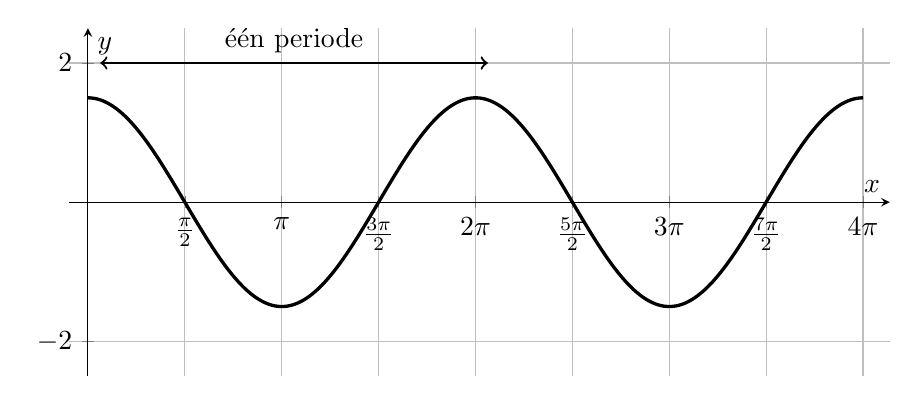
\begin{tikzpicture}
\begin{axis}[
 width=12cm,height=6cm,
 axis lines=middle,
 xmin=-0.3,xmax=13,ymin=-2.5,ymax=2.5,
 xlabel={$x$},ylabel={$y$},
 xtick={0,1.5708,3.1416,4.7124,6.2832,7.854,9.4248,10.9956,12.5664},
 xticklabels={$0$,$\frac{\pi}{2}$,$\pi$,$\frac{3\pi}{2}$,$2\pi$,
 $\frac{5\pi}{2}$,$3\pi$,$\frac{7\pi}{2}$,$4\pi$},
 grid=both,samples=250
]
\addplot[very thick,domain=0:12.5664] {1.5*cos(deg(x))};
\draw[<->,thick] (axis cs:0.2,2) -- node[above] {één periode} (axis cs:6.4832,2);
\end{axis}
\end{tikzpicture}
\end{center}

\begin{definitie}
Een functie \(f\) is \textbf{periodiek} als er een getal \(T>0\) bestaat zodat
\[
f(x+T)=f(x)
\]
voor alle \(x\) waarvoor beide functiewaarden betekenis hebben.

Zo'n \(T\) noemen we een \textbf{periode}.
\end{definitie}

De grafiek wordt dus na een horizontale verschuiving over \(T\) opnieuw dezelfde.

\FVDsection{De kleinste positieve periode}

Als \(T\) een periode is, dan zijn in de gebruikelijke periodieke situaties ook
\[
2T,\ 3T,\ 4T,\ldots
\]
periodes. Daarom zoeken we bij een niet-constante periodieke functie doorgaans
naar de \textbf{kleinste positieve periode}.

\begin{definitie}
De \textbf{fundamentele periode} is de kleinste positieve periode \(T\),
als zo'n kleinste positieve periode bestaat.
\end{definitie}

\begin{voorbeeld}
Voor
\[
f(x)=\cos x
\]
herhaalt de grafiek zich na \(2\pi\):
\[
\cos(x+2\pi)=\cos x.
\]
Ook \(4\pi\) geeft herhaling, maar is niet de fundamentele periode.
\end{voorbeeld}

\begin{opmerking}
Niet elk herhaald visueel kenmerk geeft al een volledige periode.
Twee opeenvolgende nulpunten of een maximum en het volgende minimum
liggen bijvoorbeeld niet noodzakelijk één volledige periode uit elkaar.
Vergelijk overeenkomstige punten in het patroon.
\end{opmerking}

\FVDsection{Periode aflezen uit een grafiek}

Zoek twee opeenvolgende overeenkomstige punten, bijvoorbeeld:
\begin{itemize}
  \item maximum naar volgend maximum;
  \item minimum naar volgend minimum;
  \item dezelfde middenlijnkruising met dezelfde bewegingsrichting.
\end{itemize}

Hun horizontale afstand geeft de periode.

\begin{voorbeeld}
Een periodieke grafiek heeft maxima bij
\[
x=1,\quad x=5,\quad x=9.
\]
De afstand tussen opeenvolgende maxima is \(4\). De periode is dus
\[
T=4.
\]
\end{voorbeeld}

\FVDsection{Amplitude en middenlijn}

Periodieke functies hoeven niet rond de \(x\)-as te oscilleren.

\begin{center}
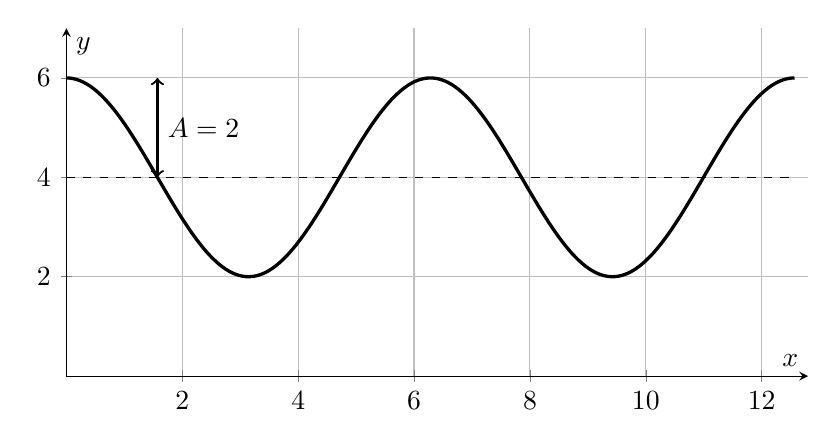
\begin{tikzpicture}
\begin{axis}[
 width=11cm,height=6cm,
 axis lines=middle,
 xmin=0,xmax=12.8,ymin=0,ymax=7,
 xlabel={$x$},ylabel={$y$},
 grid=both,samples=220
]
\addplot[very thick,domain=0:12.5664] {4+2*cos(deg(x))};
\addplot[dashed,domain=0:12.5664] {4};
\draw[<->,thick] (axis cs:1.5708,4) -- node[right] {\(A=2\)} (axis cs:1.5708,6);
\end{axis}
\end{tikzpicture}
\end{center}

Hier is de middenlijn
\[
y=4.
\]
De maximale verticale uitwijking ten opzichte van die middenlijn is \(2\).

\begin{definitie}
Voor een oscillerende functie met maximum \(M\) en minimum \(m\) is de
\textbf{amplitude}
\[
\boxed{A=\frac{M-m}{2}}.
\]
De middenwaarde is
\[
\boxed{d=\frac{M+m}{2}}.
\]
De middenlijn heeft vergelijking \(y=d\).
\end{definitie}

\begin{voorbeeld}
Als
\[
M=11,\qquad m=3,
\]
dan
\[
A=\frac{11-3}{2}=4
\]
en
\[
d=\frac{11+3}{2}=7.
\]
De functie oscilleert dus \(4\) eenheden boven en onder de middenlijn \(y=7\).
\end{voorbeeld}

\begin{opmerking}
Amplitude is geen horizontale afstand. Periode en amplitude beschrijven twee
verschillende aspecten:
\[
\boxed{\text{periode = horizontale herhaling}}
\qquad
\boxed{\text{amplitude = verticale uitwijking}}.
\]
\end{opmerking}

\FVDsection{Van één periode naar de volledige grafiek}

Als \(f\) periode \(T\) heeft, dan
\[
f(x+T)=f(x).
\]
Daaruit volgt ook
\[
f(x-T)=f(x).
\]

Kennis van één volledig periode-interval laat dus toe de grafiek naar links
en rechts te reconstrueren.

\begin{voorbeeld}
Een periodieke functie heeft periode \(6\) en
\[
f(1)=4,\qquad f(2)=-1.
\]
Dan volgt onmiddellijk
\[
f(7)=4,\qquad f(-5)=4,
\]
en
\[
f(8)=-1,\qquad f(-4)=-1.
\]
\end{voorbeeld}

\FVDsection{Periode en amplitude zijn onafhankelijk}

Twee grafieken kunnen dezelfde periode maar een verschillende amplitude hebben.
Omgekeerd kunnen twee grafieken dezelfde amplitude hebben en zich met een
verschillende periode herhalen.

\begin{center}
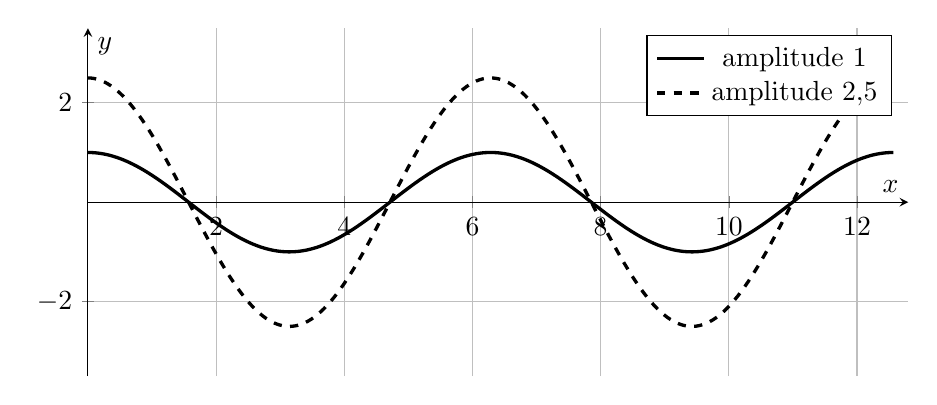
\begin{tikzpicture}
\begin{axis}[
 width=12cm,height=6cm,
 axis lines=middle,
 xmin=0,xmax=12.8,ymin=-3.5,ymax=3.5,
 xlabel={$x$},ylabel={$y$},
 grid=both,samples=250,
 legend style={at={(0.98,0.98)},anchor=north east}
]
\addplot[very thick,domain=0:12.5664] {cos(deg(x))};
\addlegendentry{amplitude \(1\)}
\addplot[very thick,dashed,domain=0:12.5664] {2.5*cos(deg(x))};
\addlegendentry{amplitude \(2{,}5\)}
\end{axis}
\end{tikzpicture}
\end{center}

Beide grafieken hierboven hebben dezelfde horizontale herhaling, maar een
verschillende verticale uitwijking.

\FVDsection{STEM-context: een periodiek signaal}

Een sensor meet een periodiek signaal. Tijdens één cyclus varieert de spanning
tussen
\[
1{,}2\ \mathrm{V}
\qquad\text{en}\qquad
4{,}8\ \mathrm{V}.
\]
Het patroon herhaalt zich om de
\[
0{,}020\ \mathrm{s}.
\]

Dan is
\[
T=0{,}020\ \mathrm{s},
\]
terwijl
\[
A=\frac{4{,}8-1{,}2}{2}=1{,}8\ \mathrm{V}.
\]
De middenwaarde is
\[
\frac{4{,}8+1{,}2}{2}=3{,}0\ \mathrm{V}.
\]

De periode zegt \emph{wanneer} het patroon zich herhaalt.
De amplitude zegt hoe groot de maximale uitwijking ten opzichte van de
middenwaarde is.

\begin{opmerking}
In fysica en techniek wordt vaak ook de frequentie gebruikt. De precieze studie
daarvan hoort bij de betrokken fysische context. Hier staat het analyseren van
de functiegrafiek centraal.
\end{opmerking}

\FVDsection{STEM-context: hoogte bij een draaiend systeem}

Een punt op de rand van een draaiend wiel beweegt periodiek omhoog en omlaag.
Als de as van het wiel \(1{,}8\) m boven de grond ligt en de straal \(0{,}6\) m is,
dan varieert de hoogte tussen
\[
1{,}2\ \mathrm{m}
\quad\text{en}\quad
2{,}4\ \mathrm{m}.
\]

De middenwaarde is
\[
1{,}8\ \mathrm{m}
\]
en de amplitude is
\[
0{,}6\ \mathrm{m}.
\]

De periode hangt af van de tijd die het wiel nodig heeft voor één volledige
omwenteling.

Dit voorbeeld toont dat amplitude en periode een concrete betekenis krijgen
wanneer we terugkeren naar de oorspronkelijke situatie.

\FVDsection{Onderzoeken met GeoGebra}

Voer in GeoGebra bijvoorbeeld in:
\[
f(x)=\cos x,
\qquad
g(x)=2\cos x,
\qquad
h(x)=\cos(2x).
\]

Onderzoek grafisch:
\begin{enumerate}
  \item welke functies dezelfde periode hebben;
  \item welke functies dezelfde amplitude hebben;
  \item wat de factor \(2\) vóór de cosinus zichtbaar verandert;
  \item wat de factor \(2\) bij \(x\) zichtbaar verandert.
\end{enumerate}

Formuleer je conclusies eerst vanuit de grafieken. De algemene theorie van
transformaties van sinusfuncties wordt later systematisch opgebouwd.

\begin{opmerking}
GeoGebra dient hier om patronen te onderzoeken en vermoedens te controleren.
Je moet periode en amplitude daarna ook zonder software uit een duidelijke
grafiek kunnen afleiden en interpreteren.
\end{opmerking}

\FVDsection{Samenvatting}

\[
\important{
\text{herhaling}
\longrightarrow
\text{periode}
\qquad\text{en}\qquad
\text{verticale uitwijking}
\longrightarrow
\text{amplitude}
}
\]

Onthoud:
\begin{itemize}
  \item \(f(x+T)=f(x)\) beschrijft periodiciteit;
  \item we zoeken doorgaans de kleinste positieve periode;
  \item vergelijk overeenkomstige punten om de periode grafisch te bepalen;
  \item \(A=(M-m)/2\);
  \item de middenwaarde is \(d=(M+m)/2\);
  \item periode is horizontaal, amplitude verticaal;
  \item één volledige periode bepaalt door herhaling de rest van een periodieke grafiek;
  \item in context moeten periode en amplitude opnieuw met eenheid en betekenis
        worden geïnterpreteerd.
\end{itemize}

\end{document}
